\documentclass[preview]{standalone}

\usepackage[usenames,dvipsnames]{xcolor}
\usepackage{tikz,ifthen,fullpage}
\usetikzlibrary{intersections}

\begin{document}
\thispagestyle{empty}

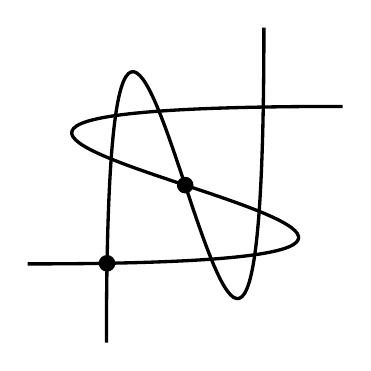
\begin{tikzpicture}
\clip (-2,-2) rectangle (2,2);
\draw [very thick, name path=curve 1] (-2,-1) .. controls (8,-1) and (-8,1) .. (2,1);
\draw [very thick, name path=curve 2] (-1,-2) .. controls (-1,8) and (1,-8) .. (1,2);
\fill [name intersections={of=curve 1 and curve 2, by={a,b}}] (a) circle (3pt)
        (b) circle (3pt);
\end{tikzpicture}
\end{document}
